% colbin: the paper. Build with `make` in this directory (see Makefile).
%
% No number in this document is typed in. Tables are \resulttable{name}, which
% reads tables/<name>.tex; a number in a sentence is \result{key}, defined in
% tables/numbers.tex. Both are written by cmd/summary from one results
% directory (`make RUN=../results/<run>` copies its tables/ here). The second
% machine's run is read the same way from tables-laptop/, as \laptoptable{name}
% and \result{laptop.key} (`make LAPTOP=../results/<run>`). A table or a key
% a run does not have prints in red and warns in the log.
\documentclass[10pt]{article}

\usepackage[T1]{fontenc}
\usepackage[utf8]{inputenc}
\usepackage{lmodern}
\usepackage[a4paper,margin=2.4cm]{geometry}
\usepackage{microtype}
\usepackage{booktabs}
\usepackage{xcolor}
\usepackage{graphicx}
\usepackage{pgfplots}
\pgfplotsset{compat=1.17}
\usepackage[hidelinks]{hyperref}
\usepackage{url}
\usepackage{placeins}

% ---- results ---------------------------------------------------------------
\makeatletter
\newcommand{\tables}{tables}
\newcommand{\resultdef}[2]{\expandafter\gdef\csname result@#1\endcsname{#2}}
\DeclareRobustCommand{\result}[1]{%
  \ifcsname result@#1\endcsname\csname result@#1\endcsname
  \else\textcolor{red}{\texttt{[#1?]}}\PackageWarning{results}{no result '#1'}\fi}
\newcommand{\resulttable}[1]{%
  \IfFileExists{\tables/#1.tex}{\input{\tables/#1.tex}}%
  {\fbox{\textcolor{red}{\texttt{\tables/#1.tex} is not in this run}}%
   \PackageWarning{results}{no table '#1'}}}
% A run that is not the paper's (cmd/summary says why) is announced on the
% first page, so a draft built on a smoke test cannot pass for the result.
\newcommand{\provisionalbanner}{%
  \ifcsname result@provisional\endcsname
    \expandafter\ifx\csname result@provisional\endcsname\empty\else
      \begin{center}\fbox{\parbox{0.92\linewidth}{\small\textcolor{red}{\textbf{Provisional numbers.}}
      The results in this draft are not the ones to publish:
      \csname result@provisional\endcsname.}}\end{center}
    \fi
  \else
    \begin{center}\fbox{\textcolor{red}{\textbf{No results:} run \texttt{make RUN=../results/<run>}.}}\end{center}
  \fi
  \ifcsname result@laptop.provisional\endcsname
    \expandafter\ifx\csname result@laptop.provisional\endcsname\empty\else
      \begin{center}\fbox{\parbox{0.92\linewidth}{\small\textcolor{red}{\textbf{Provisional numbers, second machine.}}
      \csname result@laptop.provisional\endcsname.}}\end{center}
    \fi
  \else
    \begin{center}\fbox{\textcolor{red}{\textbf{No second machine:} run \texttt{make LAPTOP=../results/<run>}.}}\end{center}
  \fi}
% The second machine's run (Section~\ref{sec:second-machine}): the same keys,
% read from tables-laptop/ and prefixed laptop., so that \result{laptop.key}
% is that machine's \result{key}; \laptoptable{name} is its \resulttable{name}.
\newcommand{\laptoptable}[1]{%
  \IfFileExists{tables-laptop/#1.tex}{\input{tables-laptop/#1.tex}}%
  {\fbox{\textcolor{red}{\texttt{tables-laptop/#1.tex} is not in this run}}%
   \PackageWarning{results}{no table 'laptop.#1'}}}
\makeatother
\IfFileExists{\tables/numbers.tex}{\input{\tables/numbers.tex}}{}
\begingroup
\renewcommand{\resultdef}[2]{\expandafter\gdef\csname result@laptop.#1\endcsname{#2}}
\IfFileExists{tables-laptop/numbers.tex}{\input{tables-laptop/numbers.tex}}{}
\endgroup
% The sweep's run (Figure~\ref{fig:sweep}), a run of its own: its keys are
% prefixed sweep-run., so that its machine.* and the rest do not replace the
% main run's. \sweepvs{table}{rows}{format} is colbin's decode-fresh factor.
\begingroup
\renewcommand{\resultdef}[2]{\expandafter\gdef\csname result@sweep-run.#1\endcsname{#2}}
\IfFileExists{tables-sweep/numbers.tex}{\input{tables-sweep/numbers.tex}}{}
\endgroup
\newcommand{\sweepvs}[3]{\result{sweep-run.sweep.#1.#2.#3.decode-fresh.factor}}

% A sentence whose wording depends on which way a number falls. Visible in a
% draft; \finaltrue hides the marks once each has been read against the final
% run.
\newif\iffinal
\finaltrue
\newcommand{\recheck}[1]{\iffinal\else{\footnotesize\color{blue} [check: #1]}\fi}

\newcommand{\colbin}{\textsf{colbin}}
\newcommand{\fmt}[1]{\textsf{#1}}
\newcommand{\code}[1]{\texttt{#1}}

% Curves of the distribution figures: one per format, when the run has it.
\newcommand{\distcurve}[3]{% style, file stem, legend
  \IfFileExists{\tables/#2.dat}{\addplot+[#1, mark=none] table[x=ratio, y=fraction]{\tables/#2.dat};\addlegendentry{#3}}{}}

\title{colbin: a compact, hybrid row-columnar serialization format with a self-describing mode}
\author{Ivan Joseph Angulo Reyna\\
  \small Independent Researcher, Peru\\
  \small \href{mailto:ivan@un.pe}{\texttt{ivan@un.pe}}}
\date{}

\begin{document}
\maketitle
\provisionalbanner

\begin{abstract}
Serialization formats for messages encode a list of records row by row,
repeating a field name (JSON) or a tag (Protocol Buffers, MessagePack, CBOR)
in every record. Columnar formats remove that repetition, but they are built
for files and analytical batches, with schemas and metadata that outweigh a
small message. \colbin{} is a hybrid binary serialization format: a message
is written in a row format with one-byte field headers, and inside it each
collection of eight or more records is written column by column, each
integer column through a per-column transform and bit-packing in
byte-aligned blocks of 128 values, a choice made per value when encoding.
\colbin{} needs
no build step: the Go struct is the schema, with no interface description
file, no schema compiler and no generated code. A message can embed its schema, a median of
\result{composition.web.tpch.schema-bytes} to
\result{composition.web.publicbi.schema-bytes} bytes by dataset, and is then
self-describing: any reader renders it as JSON without the producer's
type. We evaluate \colbin{} against \result{formats.baselines} other formats
and implementations in Go on \result{cases.total} cases from TPC-H, TPC-DS,
the Public BI Benchmark and the SchemaStore corpus, on two machines.
Compared with Protocol Buffers with the code generated by
\fmt{vtprotobuf}, \colbin{}, which generates none, is
\result{vs.categories.web-tables.vtprotobuf.gzip.factor} smaller under gzip
(\result{vs.categories.web-tables.vtprotobuf.raw.factor} as written), encodes
\result{vs.categories.web-tables.vtprotobuf.encode.factor} faster and decodes
\result{vs.categories.web-tables.vtprotobuf.decode-fresh.factor} faster on
collections of up to $2^{14}$ records, the size a web client receives, and
\result{vs.categories.bulk.vtprotobuf.gzip.factor}
(\result{vs.categories.bulk.vtprotobuf.raw.factor}),
\result{vs.categories.bulk.vtprotobuf.encode.factor} and
\result{vs.categories.bulk.vtprotobuf.decode-fresh.factor} on larger ones.
On single records, where there are no columns to write, it is the same size
under gzip (\result{vs.categories.web-documents.vtprotobuf.gzip.factor}),
decodes at the same speed
(\result{vs.categories.web-documents.vtprotobuf.decode-fresh.factor}) and
is {\let\textbf\relax
\result{vs.categories.web-documents.vtprotobuf.encode.factor}} to encode.
Against JSON, both under gzip, the collections of web size are
\result{vs.categories.web-tables.json-v2.gzip.factor} smaller
(\result{vs.categories.web-tables.json-v2.raw.factor} as written) and decode
\result{vs.categories.web-tables.json-v2.decode-fresh.factor} faster. The
format is built for collections and stays close to generated code on single
records, where Avro is smaller and generated MessagePack is faster; Arrow
and FlatBuffers read a field without decoding, which \colbin{} does not.
\end{abstract}

\section{Introduction}
\label{sec:introduction}

A response from a server to a client is, more often than not, a list of
records: the rows of a report, the products of a catalogue page, the events of
a time window. JSON~\cite{rfc8259} writes such a list with every field name in
every record and every number as decimal text. The binary formats that replace
it in practice, Protocol Buffers~\cite{protobuf}, MessagePack~\cite{msgpack}
and CBOR~\cite{rfc8949}, remove the names or shorten them, and write numbers
in binary, but they keep the row-by-row layout: a thousand records carry a
thousand copies of each field's tag, and values of one field, which resemble
each other, are separated by values of the others, which do not.

Columnar formats solved this for analytical storage long ago. Storing the
values of one column together removes the per-row tags, and lets each column
be encoded with lightweight transforms such as delta, frame of reference and
bit-packing~\cite{zukowski2006pfor,lemire2015simdbp128}, as
Parquet~\cite{parquet} and, more recently, BtrBlocks~\cite{kuschewski2023btrblocks}
and FastLanes~\cite{afroozeh2023fastlanes} do for files, and as
Arrow~\cite{arrow} does for in-memory interchange without compression. These
formats are designed for tables of millions of rows. Their framing, schema and
metadata are a fixed cost that a message of a few hundred bytes cannot
absorb, they do not carry a document that is not a table, and they come with
a schema language or a builder API that the application's own types have to
be mapped to.

This paper presents \colbin{}, a \emph{hybrid} serialization format: a
message is written in a row format, and the columnar layout is applied
inside it, where it pays, and nowhere else. The unit of decision is the
value, at encode time: a slice of structs whose fields are scalars or
strings is written as a list of rows when it is short, and as a table of
columns from eight rows up. The rest of the message, the fields of the root,
nested structs and maps, uses the row format, with one-byte field headers
and no variable-length integers. A three-field configuration document and a
million-row table are therefore the same format, and the encoder needs no
hint about which it is writing. The two halves are evaluated apart: the
single records of the evaluation measure the row format alone, and the
collections measure the columns.

The second design constraint is setup cost. The schema of a \colbin{} message
is the Go struct itself: field numbers come from optional struct tags or are
derived from field names, there is no interface description file, no compiler
step and no generated type. This is the niche of Go's
\fmt{gob}~\cite{gob,pike2011gobs}, and the reason a format with the size of a
schema-compiled one is worth having without the compilation. A message can
also carry its schema, in which case any reader renders it as JSON with no
type at hand.

\paragraph{What it is used for.} \colbin{} is a general-purpose format: any
place where Protocol Buffers or MessagePack would serve is a candidate. It
was built for one application, a business system developed by the author,
and its design follows the places where that system had JSON. They are of three kinds, and the
evaluation is organised by them.
\begin{itemize}
\item \emph{Bulk tables}: archives and backups of whole tables, written once
  and read rarely, where size is the cost.
\item \emph{Tables of web size}: the responses a server sends to a web
  client, a page of records at a time, and the cache of those responses.
\item \emph{Single records}: a record stored as one binary value in a
  key-value store, in place of a JSON document or one attribute per field,
  a small object stored in a binary column of a relational table, where a
  JSON or text column would otherwise hold it, and a message between two
  services.
\end{itemize}
The row format's narrow field header, one byte for a type of up to sixteen
fields (Section~\ref{sec:format}), exists for the last kind: the small
objects that end up as a field of a larger record are, in a database,
usually a JSON string, and most of such a string is field names and
punctuation. A format that is to replace JSON in all three places has to
be cheap for an object of three fields and compact for a table of a
million rows, which is the choice per value described above.

\paragraph{Contributions.}
\begin{itemize}
\item A hybrid message format in which a slice of structs is a list of rows
  or a columnar table, decided per value, with integer columns encoded by a
  per-column transform and bit-packed in byte-aligned blocks of 128 values,
  and float columns encoded as decimals where they are decimals
  (Section~\ref{sec:format}).
\item A row format for everything that is not a table: one byte of header
  per field for types of up to sixteen fields, zero values not written, and
  every size read with a single load rather than a variable-length loop.
\item A self-describing mode: a message can embed its schema, a key, a name
  and an operation code per field, and any reader then renders it as JSON,
  or decodes it into another type by field name, without the producer's
  type. Its cost is measured against the message it describes
  (Section~\ref{sec:composition}).
\item An evaluation in Go against \result{formats.baselines} formats and
  implementations (JSON, \fmt{gob}, CBOR, MessagePack, Protocol Buffers with two
  implementations, FlatBuffers, Arrow IPC, Avro and Cap'n Proto), raw and
  under gzip and Zstandard, on \result{cases.total} cases from four
  public sources, none of them designed by the author
  (Sections~\ref{sec:methodology} and~\ref{sec:results}).
\item Ablations of the two parameters the layout rests on: the row count at
  which a slice becomes a table, and the choice of column transform
  (Section~\ref{sec:ablations}).
\item An account of where the format loses or ties, and of what the
  evaluation does not cover (Section~\ref{sec:limitations}).
\item A reproducible artifact: datasets pinned by checksum, the exact subset
  rules, and one command that regenerates every table and figure of this
  paper (Section~\ref{sec:availability}).
\end{itemize}

The evaluation compares \colbin{} with each other format directly, on the
cases both carry, and reports the comparison two ways: by dataset, and by
the three kinds of message above. A response to a web client bounds the
size of a message, so a table of web size is one of at most $2^{14}$ rows
and a bulk table one past that bound; a single record is a document that
holds no table.

\section{The format}
\label{sec:format}

This section describes the wire format at the level the evaluation needs. The
byte-level specification, and the measurements behind each decision, are in
the library's repository (Section~\ref{sec:availability}).

\subsection{Messages are key runs}

A message is a \emph{key run}: a sequence of fields, each a key, a descriptor
and a payload, ended by the length of whatever encloses it. A run uses one of
two key widths, chosen per struct type and recorded where the run opens. In
the narrow width a field header is a single byte, four bits of key and four
of descriptor, which covers types whose field numbers are 1 to 16. In the wide
width it is two bytes, eight bits each, for numbers up to 255; a type with
more fields is split into linked pages of 255. A nested struct opens its own
run, so narrow and wide types nest in either order. In both widths the
descriptor is enough to step over a field the reader does not know, so
producer and consumer can add and drop fields independently.

Field numbers come from a struct tag (\code{cb:"3"}) or, without one, from an
8-bit hash of the field's name with linear probing on collision. Untagged
types therefore always use the wide width and cost one more byte per field
present, and are limited to 255 fields. Tags are optional; every type in the
evaluation has them.

\subsection{Scalars}

A field holding its type's zero value is not written. An integer is written as
sign and magnitude in the fewest bytes that hold it, one to eight, with the
byte count in the descriptor; in the narrow width, the values the descriptor
itself can name (1 to 4, or 1 to 3 and $-1$ for a signed field) need no
payload, so a boolean or a small enumeration is one byte with its key. A
string of up to eight bytes takes its size from the descriptor; a longer one
carries a length of one, three or five bytes.

No size anywhere in the format is a variable-length integer. Protocol
Buffers' varints are compact, but each is decoded by a loop whose trip count
is data, a cost that byte-oriented schemes such as Stream
VByte~\cite{lemire2018streamvbyte} exist to avoid. In \colbin{} every read of
a size is one load of a width the header has already given.

A scalar floating-point field is written as its IEEE~754 bit pattern with the
bytes reversed, in the unsigned integer form. The zero bytes of a float are
its low mantissa bytes, where an integer's are its high ones, so the trim that
shortens an integer shortens a round float too: \code{1.0} is two bytes.

\subsection{Composites, lists and tables}

A nested struct, a list, a table or a map is written with its byte length in
front, patched in after the body is written, which is what lets a reader skip
it whole. A nil pointer is omitted; a pointer to a zero value is the one case
in which the format writes a zero, to keep the two apart.

A slice of structs is written in one of two layouts
(Figure~\ref{fig:layouts}):
\begin{itemize}
\item as a \emph{list}, each element its own key run, when it has fewer than
  eight elements, or when the element type holds something that is not a
  column (a map, a nested struct, a slice of scalars);
\item as a \emph{table}, when it has at least eight elements and every field
  of the element type is a boolean, an integer, a float, a string, a pointer
  to one of those, or itself a slice of structs that qualifies.
\end{itemize}
The decision is taken per value at encode time, and the two layouts have
different descriptors, so a reader dispatches on what it finds and neither
side is configured. A table writes one key per column instead of one per field
per row. A nullable column (a pointer field, which is how a Go type says a value
may be absent) carries one bit of presence per row and the values of the rows
present only, so the column codec sees real values and a run of nulls costs a
bit a row; a column whose values are all zero, or all null, is not written at
all. A table of more than 4\,096 rows is
written in groups of 4\,096 rows, each group a complete set of columns, which
bounds the memory the encoder transposes through and keeps a group's columns
in cache. The threshold of eight rows is the subject of the first ablation in
Section~\ref{sec:ablations}.

\begin{figure}[t]
\centering\small
\begin{tabular}{@{}l@{\qquad}l@{}}
\textbf{list} (fewer than 8 rows) & \textbf{table} (8 rows or more)\\[2pt]
\code{[len]} & \code{[len][rows]}\\
\code{\ \ [len] k1 v k2 v k3 v} & \code{\ \ k1 [column: v v v v ...]}\\
\code{\ \ [len] k1 v k2 v k3 v} & \code{\ \ k2 [column: v v v v ...]}\\
\code{\ \ [len] k1 v k2 v k3 v} & \code{\ \ k3 [column: v v v v ...]}\\
\end{tabular}
\caption{The two layouts of a slice of structs with three fields. A list
repeats each key in every row; a table writes each key once and its values
together, where a column transform can use what they have in common.}
\label{fig:layouts}
\end{figure}

\subsection{The column codec}
\label{sec:column-codec}

An integer column (and a boolean, date or timestamp column, which are integer
columns) is one transform followed by blocks of bit-packed residuals:
\begin{itemize}
\item \emph{raw}: the values, zigzag-encoded if any is negative;
\item \emph{delta}: differences between consecutive values, zigzag-encoded,
  after the first value;
\item \emph{frame of reference}: each value minus the column's
  minimum~\cite{zukowski2006pfor};
\item \emph{constant}: the single value, and no blocks.
\end{itemize}
The encoder scores each candidate by the bytes its blocks would occupy and
keeps the smallest. Residuals are then packed in blocks of 128 values, each
block at its own bit width, written in one byte ahead of it. The block size is
that of SIMD-BP128~\cite{lemire2015simdbp128}, and it is chosen for the same
arithmetic: 128 values of $w$ bits are exactly $16w$ bytes, so every block
starts and ends on a byte boundary, no state crosses from one block to the
next, and one outlier widens 128 values rather than the column. A block of
zeros has width 0 and costs one byte. Unpacking is one unaligned 8-byte load,
a shift and a mask per value for widths up to 57 bits, with the width switched
on once per block; there is no patching of exceptions as in PFOR. The second
ablation in Section~\ref{sec:ablations} forces each transform in turn.

A column of 64-bit floats whose values are decimals, as most floats that
came out of a database or a CSV file are, is written as integers: the encoder
looks for one exponent $e$ per column such that $v \cdot 10^e$ is an integer
that converts back to $v$ exactly, writes those integers through the integer
codec, and keeps the values that do not fit as exceptions with their position
and bit pattern. This is the decimal half of ALP~\cite{afroozeh2023alp} with
one exponent per column and a division on decode rather than a multiplication
by the inverse, which is slower but exact on every platform. The column is
written this way only when it is smaller than the bit patterns would be.

String columns are written as the strings one after another, each with its
size; they are not dictionary-coded.

\subsection{Optional parts}

\paragraph{The schema section.} The wire carries no names and no types. A
\emph{schema section}, the type's encoding plan serialized as a key, a name
and an operation code per field, can be sent once per connection, or embedded
at the front of a message. With it embedded, the message is self-describing:
it can be rendered as JSON, or decoded into a different type by matching
field names, with no knowledge of the producer's type. The evaluation
measures this mode as \fmt{colbin-json}, and reports the size of the section
against the message in Section~\ref{sec:composition}.

\paragraph{Dynamic values.} A field of an open type (Go's \code{any},
\code{[]any}, \code{map[string]any}) is written with a type descriptor per
value, as schemaless formats do. No case of the evaluation uses this path.

\paragraph{packed5.} An opt-in encoding packs strings of letters and digits
at about five bits per character, when that is shorter. It is off by default
and reported as a separate variant, \fmt{colbin+packed5}.

\subsection{Schema evolution}
\label{sec:evolution}

The writer's type and the reader's need not be the same type. A field is
found by its key, and a key the reader does not know is stepped over by its
descriptor, so a field can be added or removed on either side: the reader
of an older message finds the new field at its zero value, and the reader of
a newer one skips what it does not know. The same holds for a column of a
table, which is one key for all its rows. With tags the key is the tag, so a
field can be renamed freely; without them the key is a hash of the name, and
a renamed field is another field. An integer is written by its value, not by
its declared width, so a field can be widened (an \code{int32} read as an
\code{int64}) or narrowed, as long as the values fit.

Table~\ref{tab:evolution} sets this beside the two formats the evaluation
compares \colbin{} with most closely. It is close to Protocol Buffers'
rules~\cite{protobuf}, with tags in the place of field numbers, and with two
differences against \colbin{}. A value that does not fit the reader's
narrower integer is an error in a record but is truncated without one in a
column, where the check is not made per value. And a change of kind, an
integer to a float or to a string, is not supported and is not always
detected: the reader may return a wrong value instead of an error.
Protocol Buffers also keeps the unknown fields of a message it decodes and
writes again; \colbin{} drops them. The behaviour of \colbin{} in the table
is checked by a test in the artifact (\code{formats/evolution\_test.go});
that of the other two is their documentation's, and for MessagePack's
integers the same test.

\begin{table}[t]
\centering\footnotesize
\begin{tabular}{@{}p{0.23\linewidth}p{0.25\linewidth}p{0.21\linewidth}p{0.21\linewidth}@{}}
\toprule
change & \colbin{} & Protocol Buffers & MessagePack (generated, keyed by name) \\
\midrule
a field or a column added or removed & compatible both ways & compatible both ways & compatible both ways \\
a field renamed & compatible with tags; another field without & compatible & another field, unless a tag keeps the name \\
an integer widened & compatible & compatible & compatible \\
an integer narrowed, a value out of range & error in a record; truncated in a column & truncated & error \\
a change of kind (integer to float or string) & not supported, not always detected & not compatible & error \\
\bottomrule
\end{tabular}
\caption{What a reader sees when its type is not the writer's. \emph{Compatible
both ways}: an old reader decodes a new message and a new reader an old one,
with the missing field at its zero value.}
\label{tab:evolution}
\end{table}

\subsection{Implementation}

The Go implementation has no dependencies. It builds an encoding plan per
type on first use, by reflection, and then runs it over unsafe pointers, so
the steady state involves no reflection except for maps. The hot loops of the
column codec have assembly kernels on amd64 and arm64. Decoders treat their
input as hostile: every length, count and row total is bounded before
anything is allocated. Implementations in Rust and in JavaScript (through
WebAssembly) read and write the same bytes; this paper evaluates the Go
implementation only.

\section{Related work}
\label{sec:related}

\paragraph{Serialization formats.} The formats \colbin{} is compared with fall
in three groups. Schemaless formats, MessagePack~\cite{msgpack} and
CBOR~\cite{rfc8949}, are binary JSON: they keep field names in every record.
Schema-driven row formats, Protocol Buffers~\cite{protobuf} and
Avro~\cite{avro}, remove the names; Protocol Buffers keeps a tag per field,
which makes fields optional and skippable, and Avro keeps nothing, which makes
it the smallest row format and ties reader and writer to the same schema.
Zero-copy formats, FlatBuffers~\cite{flatbuffers} and Cap'n
Proto~\cite{capnproto}, lay a message out so that a field is read in place,
at the price of fixed-width fields and alignment. Go's
\fmt{gob}~\cite{gob,pike2011gobs} is the format closest to \colbin{} in how it
is used: it takes its schema from the Go type and needs no compilation, and it
sends type descriptions in the stream. All of these write a list of records
row by row.

\paragraph{Benchmarks of serialization formats.} Viotti and Kinderkhedia
survey JSON-compatible binary formats~\cite{viotti2022survey} and benchmark
their sizes on 27 real documents taken from
SchemaStore~\cite{viotti2022benchmark,schemastore}, later extended to JSON
BinPack~\cite{viotti2022binpack}. We use their corpus unchanged, as the
representative of small, heterogeneous documents, where a columnar layout has
nothing to work with. Their study measures size only; we add encode and decode
time. HyperProtoBench~\cite{karandikar2021protoacc} characterises Protocol
Buffers workloads at a large operator and motivates hardware acceleration of
varint and field decoding, the per-field costs that \colbin{}'s fixed-width
sizes are meant to avoid in software.

\paragraph{Lightweight integer compression.} The column codec belongs to the
family of frame-of-reference and bit-packing schemes. PFOR and
PFOR-DELTA~\cite{zukowski2006pfor} introduced patched frame of reference with
decoding loops free of data-dependent branches. Lemire and
Boytsov~\cite{lemire2015simdbp128} showed that bit-packing blocks of 128
integers at one width per block decodes at billions of integers per second
with SIMD; \colbin{} uses their block size and its byte alignment, without
exceptions and with scalar unpacking. Stream
VByte~\cite{lemire2018streamvbyte} addresses the cost of variable-length
integers by separating control bytes from data; \colbin{} avoids such
integers altogether. FastLanes~\cite{afroozeh2023fastlanes} goes further than
any of these with a layout that auto-vectorizes across instruction sets.
\colbin{}'s codec is deliberately simpler than the state of the art: it has to
pay for itself on a column of eight values as well as on one of a million.

\paragraph{Floating-point compression.} Gorilla~\cite{pelkonen2015gorilla}
and Chimp~\cite{liakos2022chimp} XOR consecutive values of a time series.
ALP~\cite{afroozeh2023alp} observes that most doubles in real data are
decimals and encodes them as integers. \colbin{} adopts ALP's decimal
encoding in a reduced form (Section~\ref{sec:column-codec}).

\paragraph{Columnar formats and nested data.} Dremel~\cite{melnik2010dremel}
showed how to shred nested records into columns with repetition and definition
levels, the basis of Parquet~\cite{parquet}. Arrow~\cite{arrow} defines a
columnar memory layout and an IPC stream for it. BtrBlocks~\cite{kuschewski2023btrblocks}
selects among cascades of lightweight encodings per column block by sampling,
and Zeng et al.~\cite{zeng2023columnar} evaluate Parquet and ORC and find
their encodings dated against such schemes. JSON
Tiles~\cite{durner2021jsontiles} extracts columnar structure from collections
of JSON documents inside a database. These systems target storage and
analytics: data at rest, read many times, in files whose footers and
dictionaries are amortised over millions of rows. \colbin{} targets a message
produced once and read once, usually small, in which a table is one field
among others; it does not shred nested records, but lets a row hold a list
column whose elements are again rows. Mixing the two layouts is not new in
storage: PAX~\cite{ailamaki2001pax} keeps a relation in row pages and lays
each page out by column. There the mix is fixed by the storage layout; in
\colbin{} it is decided per value while a message is encoded, and a message
with no collection in it has no columnar part at all.

\paragraph{Benchmark data.} TPC-H~\cite{tpch} and
TPC-DS~\cite{tpcds,nambiar2006tpcds} are generated from near-uniform
distributions, and Vogelsgesang et al.~\cite{vogelsgesang2018getreal} show
how poorly such data represents real workloads for encodings. The Public BI
Benchmark~\cite{publicbi,ghita2020whitebox}, derived from real Tableau
workbooks, is the corrective used in the compression literature, including by
BtrBlocks and ALP, and it is here as well.

\section{Methodology}
\label{sec:methodology}

\subsection{What is evaluated}

\colbin{} is evaluated as a serialization format in Go: the bytes a Go
program writes and reads, against the Go implementations of the other
formats. One of its uses is a server's response to a web client in place of
JSON, but decoding in a browser is a different implementation and is outside
this paper; nothing here should be read as a claim about it.

\subsection{Datasets}
\label{sec:datasets}

All data is public and none of it was designed for this evaluation. Nothing
downloaded is stored in the repository: each dataset has a script that
downloads or generates it and checks every file against a manifest of SHA-256
checksums before anything reads it.

\begin{description}
\item[TPC-H]~\cite{tpch} at scale factor 0.1, generated by \code{dbgen}
  2.17.3: all eight tables, each as a case, and two composite cases, the
  whole schema as one message (\emph{normalized}) and orders with their line
  items nested inside them (\emph{nested}), the only parent and child the
  schema has.
\item[TPC-DS]~\cite{tpcds} at scale factor 0.1: all 24 tables, one case
  each.
\item[Public BI Benchmark]~\cite{publicbi}: the first table of each of the 46
  workbooks, and from each a seeded uniform random sample whose size depends
  on the table's place in the list: 350 rows of the first table by name, 700
  of the second, and so on in steps of 350, the last at $2^{14}$; or the
  whole table where it is shorter.
\item[SchemaStore]~\cite{schemastore}: the 27 documents of Viotti and
  Kinderkhedia's corpus~\cite{viotti2022benchmark}, each through a Go struct.
\end{description}

\paragraph{How the subsets are chosen.} Each subset follows a rule fixed in
the repository (\code{datasets/README.md}), not a selection of tables or rows.
For TPC-H and TPC-DS the rule is everything at one scale factor; scale factor
0.1 is about 100\,MB of text per benchmark, which every format holds in memory
at once, and a larger scale would add rows to the bulk regime only. For Public
BI the rule is the first table of every workbook, so that no workbook weighs
more than another; in 38 of the 46 workbooks it is the only table or the
others share its schema. The sizes are staggered so that the tables of web
size cover the whole range a response has, from a page of a few hundred
records to the regime's bound, rather than all sitting at that bound, where
a columnar layout is at its best; which table gets which size is decided by
its name alone. The rows are a random sample rather than the head of the file because
these tables are often sorted by their leading columns, so the head repeats
values more than the table does, which would flatter every format that
exploits repetition, \colbin{} most of all. The sample depends only on
fixed seeds, the table's name and the row index, and keeps table order: the
dataset's script draws $2^{14}$ rows of each table, and the case keeps a
second, independent draw of those. For
SchemaStore the selection is that of the corpus's authors.

\paragraph{Go types.} Every format is driven from one Go struct per dataset
root, written as a Go programmer would write it and not as any format
prefers: the narrowest integer type that holds the column per the source's
schema, money and decimals as integer minor units, dates as integer days, a
float only where the source has a float, and a pointer for a nullable column.
The schemas of the other formats (\code{.proto}, FlatBuffers, Cap'n Proto and
Avro schemas, generated MessagePack code, Arrow builders) are generated from
those structs. For TPC-H, TPC-DS and Public BI the structs themselves are
generated from the sources' \code{CREATE TABLE} statements. For SchemaStore
they were written by hand, from the Protocol Buffers schemas the corpus
provides; this is a place where the author's judgement enters
(Section~\ref{sec:limitations}).

\subsection{Kinds of message}
\label{sec:kinds}

We take $2^{14}$ rows as the bound of what a server sends to a web client in
one response; the bound is a convention of this paper, not a measurement.
Every case falls in one of two regimes by its row count alone:
\emph{web}, at most $2^{14} = 16\,384$ rows, and \emph{bulk}, more than that.
The web regime has \result{cases.web} cases: the \result{cases.web.publicbi}
Public BI samples, the \result{cases.web.schemastore} SchemaStore documents,
\result{cases.web.tpcds} TPC-DS tables and \result{cases.web.tpch} TPC-H
tables. The bulk regime has \result{cases.bulk}: the other
\result{cases.bulk.tpcds} TPC-DS tables, and for TPC-H four tables and the
two composite cases. The web regime holds two kinds of message that a
format treats differently, and the results keep them apart: a \emph{web
table}, a slice of rows (TPC-H, TPC-DS and Public BI;
\result{cases.categories.web-tables} cases), and a \emph{single record}, one
object with no table in it (SchemaStore;
\result{cases.categories.web-documents}). With \emph{bulk}
(\result{cases.categories.bulk}), these are the three kinds of message the
results are reported by, beside the four datasets, and the three uses the
format was built for (Section~\ref{sec:introduction}). SchemaStore's
documents are configuration files, not database records; they stand in for
the single record as the public corpus of small typed objects the
evaluation could use.

\subsection{Baselines}

Table~\ref{tab:baselines} lists the formats, their Go implementations and the
versions measured. Two formats appear with two implementations, because the
implementation moves the time by more than the format does: Protocol Buffers
with the reflection-based \fmt{protobuf-go} and with the generated code of
\fmt{vtprotobuf}~\cite{vtprotobuf}, and MessagePack with generated code and
with reflection. \colbin{} appears as three variants: the default
(\fmt{colbin}), with \fmt{packed5} on, and self-describing with its schema
section embedded (\fmt{colbin-json}). Only \fmt{colbin}, the default, is the result of this
paper; the others isolate one option each.

\begin{table}[t]
\centering\small
\resulttable{baselines}
\caption{Formats, implementations and versions. The versions are those pinned
by the artifact's \code{go.mod}; \colbin{}'s is the one the run recorded.}
\label{tab:baselines}
\end{table}

Not every format carries every case, and a format that cannot carry a case is
reported as not applicable, with the reason, rather than forced or silently
dropped (Table~\ref{tab:coverage}). Arrow carries only roots that are tables.
\colbin{} itself cannot carry
\result{coverage.web.colbin.na} of the 27 SchemaStore documents: it
refuses a struct with no field it can encode, and in those documents a type
has none. Cap'n Proto does not carry two SchemaStore documents, in which a
field's name collides with a method its Go code generator emits. \fmt{gob} does not transmit a pointer to a zero value, so it does
not round-trip any table with a nullable column that holds a zero; its sizes
on those cases are reported, flagged as lossy, and it is not timed on them
(Section~\ref{sec:limitations}).

\begin{table}[t]
\centering\small
\resulttable{coverage}
\caption{Cases per format and regime: round-tripped exactly, encoded but not
round-tripped (lossy; sized, not timed), and not applicable.}
\label{tab:coverage}
\end{table}

\subsection{What is measured}

\paragraph{Correctness first.} Before a size or a time is recorded, each
format encodes the case, decodes it, and the result is compared with the
original value by deep equality; where a case has an access aggregate, each
format's result is compared with the one computed on the Go value. A format
that fails a check on a case has no time for it.

\paragraph{Size.} The encoded message in bytes, as written and under two
general-purpose compressors at level 6: gzip~\cite{rfc1952}, which every
browser accepts and every server can apply to a response on the fly, and
Zstandard~\cite{rfc8878}. The text and the figures quote gzip; the tables
give both. Compressed sizes matter
because the realistic alternative to a binary format on the web is not JSON
but compressed JSON.

\paragraph{Time.} Four operations per format and case:
\emph{encode} into a reused buffer; \emph{decode-fresh}, into a value
allocated for the call; \emph{decode-reuse}, into one value held across
calls, which lets a decoder reuse its allocations; and \emph{access}, the sum
of one numeric column computed from the encoded bytes, in place where the
format allows it (Arrow, FlatBuffers, Cap'n Proto) and by decoding first
where it does not. Access is defined for the cases that have such a column
(\result{time.web.access.cases} of the web cases and
\result{time.bulk.access.cases} of the bulk cases).
For code-generated formats, converting between the format's own types and the
Go struct is outside the timed region.

\paragraph{Protocol.} Each case runs in its own process, pinned to one
hardware thread of a physical core with \code{taskset} and
\code{GOMAXPROCS=1}; the garbage collector is at its default setting, and
the runtime releases free memory to the kernel lazily
(\code{GODEBUG=madvdontneed=0}), for the reason given below. Web
cases run two at a time on two cores, bulk cases one at a time. Within a
case, every format and operation is checked and warmed up, the core is kept
busy for 200\,ms so that its clock is up before the first sample, and then
samples are taken, each after an untimed run of its own operation, round-robin over all formats and operations, so that each
benchmark sees the same neighbours and the same drift. A benchmark is
\result{machine.count} samples of at least \result{machine.sample} each, and
its value is their median. Sizes do not depend on the machine and are
computed in a separate stage.

\paragraph{Memory handed back between samples.} A process holds every
format's values of a case at once, and between two samples Go's runtime
returns free heap to the kernel. With its default on Linux
(\code{MADV\_DONTNEED}) the next benchmark that allocates takes a page
fault for every page it gets back, so what a decode into a fresh value cost
depended on which benchmark ran before it, and the round-robin order, being
fixed, repeated that in every round and in both passes. A first version of
this evaluation was measured that way, and the same decoder on the same
bytes, \colbin{}'s default and its variants, differed by up to a half on a
bulk case in decode-fresh while agreeing in decode-reuse, which allocates
nothing. Two things remove it. With \code{MADV\_FREE} the kernel takes
the pages only when it is short of memory, and the faults do not occur.
And every sample is preceded by an untimed run of the same operation for the
same time, followed by a collection, so that the memory a sample allocates
from is memory its own format has just used and freed, not another's.
\colbin{}'s variants, which share a decoder,
are in the timing tables of Appendix~\ref{sec:against-json} as the control
of this.

\paragraph{Summaries.} The results compare \colbin{} with each other format
directly: on each case both carry, \colbin{}'s number is divided by the
other format's for the same case and operation. A summary over cases is the
geometric mean of those ratios, in which every case weighs the same, with
the number of cases \colbin{} wins outright beside it. It is printed as a
factor, the inverse of that mean where \colbin{} wins ($2.5\times$ smaller,
or faster, for a mean of 0.4) and the mean itself, marked \emph{worse},
where it loses; the mean of the inverses is the inverse of the mean, so
this is the same statistic read the other way. The cases are
grouped two ways, each case in exactly one group: by dataset, and by kind of
message (Section~\ref{sec:kinds}). Because the comparison is always on the
cases both formats carry, a format that carries few cases is compared with
\colbin{} on those cases only. Each format against JSON, over the cases the
format carries and by regime, is in Appendix~\ref{sec:against-json}; there,
for access, which JSON does not have, the reference is JSON's decode-fresh,
what a client without it does instead. A message of zero bytes (a document
whose values are all defaults is zero bytes in \colbin{} and Protocol
Buffers) has a ratio of zero, which a geometric mean cannot hold; such cases
are left out of the mean and marked.

\FloatBarrier
\subsection{Machine and repeatability}
\label{sec:machine}

{\sloppy The main numbers were measured in Oracle Cloud Infrastructure container
instances of shape \code{CI.Standard.E4.Flex}, 4 OCPUs (physical cores
dedicated to the instance) and 32\,GB, on an \result{machine.cpu},
\result{machine.kernel}, Go \result{machine.go-version}, on CPUs
\result{machine.measured-cores}. Each dataset was measured in its own
instance, all four of the same shape and at the same commit, side by side;
every case, and so every ratio between two formats, comes from a single
process on a single core. Each instance was started from a pinned container
image, cloned this artifact at the commit it reports, and fetched and
verified its dataset itself.\par}

A container cannot fix the clock: the frequency governor and the boost are
the host's, and how far a core boosts depends on what the host's other
tenants do. We therefore measured the clock instead of fixing it. Before
every round of a case's samples, the harness times a chain of dependent
64-bit multiplies on the measured core, which runs at one multiply per three
cycles on this processor. Over the first web pass the clock was between
\result{probe.web.mhz.p5} and \result{probe.web.mhz.p95}\,MHz (5th and 95th
percentiles; median \result{probe.web.mhz.median}). The container exposes no other measure of the
clock: no frequency driver, no APERF/MPERF counters, a time-stamp counter
that runs at the nominal frequency, and no access to the cycle counter. The
absolute clock rests on the multiplier's documented latency; the variation,
which is what the ratios depend on, does not. Within a case, which is
what a ratio between two formats depends on, the slowest probe was within
\result{probe.web.spread.median}\,\% of the fastest for the median case and
within \result{probe.web.spread.p90}\,\% for nine cases in ten;
\result{probe.web.spread.over5} of \result{probe.web.cases} cases saw the
clock move by more than 5\,\%. Because samples are taken round-robin, such a
change falls on every format of the case alike. The probes, the machine
description and the per-second log of the cores are part of the artifact.

\paragraph{A second machine.} The same commit was measured again, in full, on
a machine of another kind: a laptop whose processor is a \result{laptop.machine.cpu}, a
15\,W client processor with two performance cores and eight efficiency
cores, \result{laptop.machine.kernel}, Go \result{laptop.machine.go-version}.
There the clock could be fixed rather than measured. Boost was disabled and
the \code{performance} governor set, so that the performance cores ran at
their base frequency throughout; the cases ran on one hardware thread of each
performance core (CPUs \result{laptop.machine.measured-cores}), with the
same protocol as above, and every other process and every interrupt were
confined to the efficiency cores. On this machine the processor's cycle
counter can be read, and it confirms the probe: over the first web pass the
probe read a median of \result{laptop.probe.web.mhz.median}\,MHz and the
cycle counter \result{laptop.probe.web.counted-mhz.median}\,MHz, at
\result{laptop.probe.web.cycles-per-multiply} cycles per multiply. Within a
case the probe moved by at most \result{laptop.probe.web.spread.p90}\,\% for
nine cases in ten, and by more than 5\,\% in
\result{laptop.probe.web.spread.over5} of \result{laptop.probe.web.cases}.
The two machines are reported apart and never pooled
(Section~\ref{sec:second-machine}); a number that does not say otherwise is
the cloud's.

The web cases were timed twice, several hours apart, to measure how far a
number moves when nothing changes. Of \result{repeat.lines} benchmarks,
\result{repeat.within3}\,\% differ by at most 3\,\% between the two passes,
\result{repeat.within5}\,\% by at most 5\,\% and \result{repeat.within10}\,\%
by at most 10\,\%; the median difference is \result{repeat.median}\,\%, the
90th percentile \result{repeat.p90}\,\%, and neither pass is slower than
the other overall. Absolute times on
this machine are therefore not repeatable to 3\,\%. Ratios between formats
are: the geometric means of each format's
time over \colbin{}'s differ between the two passes by at most
\result{repeat.ratio-worst}\,\% (Table~\ref{tab:repeatability}), because the
round-robin sampling exposes every format in a case to the same conditions.
For that reason this paper reports ratios, not absolute times, and treats a
difference between two formats smaller than about 4\,\% as no difference.
Timing tables use the first pass. On the laptop, with its clock fixed,
\result{laptop.repeat.within3}\,\% of \result{laptop.repeat.lines} benchmarks
differ by at most 3\,\% between the two passes, the median difference is
\result{laptop.repeat.median}\,\%, and the geometric means over \colbin{}'s
differ by at most \result{laptop.repeat.ratio-worst}\,\%.

\begin{table}[t]
\centering\small
\resulttable{repeatability}
\caption{Each format's time over \colbin{}'s, as a geometric mean over the
web cases both have, in the two timing passes.}
\label{tab:repeatability}
\end{table}

\section{Results}
\label{sec:results}

Every table in this section is a geometric mean of ratios against JSON on
the same case unless it says otherwise; below 1 is smaller or faster than
JSON. The \emph{cases} column is the number of cases the format has a
result for.

\FloatBarrier
\subsection{Size}
\label{sec:size}

\begin{table}[t]
\centering\small
\resulttable{sizes-web}
\caption{Web regime: message size against JSON's, as written (\emph{raw})
and under each compressor, both sides compressed alike. $\dagger$: cases
where the format writes zero bytes are left out of the mean.}
\label{tab:sizes-web}
\end{table}

\begin{table}[t]
\centering\small
\resulttable{sizes-bulk}
\caption{Bulk regime: message size against JSON's.}
\label{tab:sizes-bulk}
\end{table}

\paragraph{Web regime (Table~\ref{tab:sizes-web}).} As written, a \colbin{}
message is \result{size.web.colbin.raw} of the JSON's size, against
\result{size.web.protobuf.raw} for Protocol Buffers,
\result{size.web.msgpack.raw} for MessagePack and \result{size.web.avro.raw}
for Avro. Compression narrows every gap, because a general-purpose
compressor removes much of the redundancy a binary format removes by
construction: under brotli 5 the same four are \result{size.web.colbin.br5},
\result{size.web.protobuf.br5}, \result{size.web.msgpack.br5} and
\result{size.web.avro.br5}. The schemaless formats, and the zero-copy ones,
are within a few percent of compressed JSON: once a server compresses its
responses, they save almost nothing on the wire.
\recheck{the three sentences above describe run1; confirm direction for the
schemaless and zero-copy formats}

\paragraph{Bulk regime (Table~\ref{tab:sizes-bulk}).} With more rows per
table the column layout has more to work with: \colbin{} is
\result{size.bulk.colbin.raw} of JSON as written and
\result{size.bulk.colbin.br5} under brotli 5, where the row formats stay
close to compressed JSON (\result{size.bulk.protobuf.br5} for Protocol
Buffers, \result{size.bulk.avro.br5} for Avro) and Arrow, columnar but
uncompressed, is at \result{size.bulk.arrow.br5}. The column transforms and
the general-purpose compressor are complementary rather than redundant:
delta and frame of reference expose regularities across rows that a
byte-oriented compressor with a bounded window does not find in a row
layout. \recheck{complementarity claim: holds if colbin's br5 ratio is well
below the row formats'}

\begin{table}[t]
\centering\footnotesize
\resulttable{sizes-datasets-web}
\caption{Web regime by dataset: size against JSON's, as written and under
brotli 5.}
\label{tab:sizes-datasets-web}
\end{table}

\paragraph{By dataset (Table~\ref{tab:sizes-datasets-web}).} The mean over
the web regime hides how different its datasets are. On the tabular datasets
\colbin{} is at \result{size.web.tpcds.colbin.br5} (TPC-DS) and
\result{size.web.publicbi.colbin.br5} (Public BI) of brotli-compressed JSON.
On SchemaStore's typed documents, which are small and hold no table, it is
at \result{size.web.schemastore.colbin.br5}, beside
\result{size.web.schemastore.protobuf.br5} for Protocol Buffers and
\result{size.web.schemastore.avro.br5} for Avro: here the three schema-driven
formats do the same thing, and the result is a tie decided by a few bytes
per message. On the dynamic path, where \colbin{} writes field names like
any schemaless format, it is at \result{size.web.schemastore-dynamic.colbin.br5}.
Arrow on SchemaStore shows the fixed cost of a format made for large tables
on a message of a few hundred bytes. The bulk regime by dataset is in the
artifact (\code{tables/sizes-datasets-bulk.tex}).
\recheck{``tie'' on SchemaStore typed; which of colbin / avro is ahead}

\begin{figure}[t]
\centering
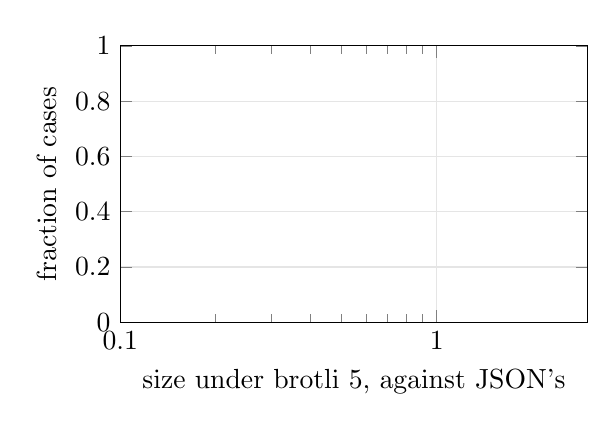
\begin{tikzpicture}
\begin{axis}[width=0.62\linewidth, height=0.42\linewidth,
  xlabel={size under brotli 5, against JSON's}, ylabel={fraction of cases},
  xmode=log, log ticks with fixed point, xmin=0.1, xmax=3, ymin=0, ymax=1,
  legend pos=outer north east, legend style={font=\footnotesize, draw=none},
  cycle list name=color list, grid=major, grid style={gray!20}]
\distcurve{very thick, black}{fig-dist-web-br5-colbin}{colbin}
\distcurve{thick, blue}{fig-dist-web-br5-protobuf}{protobuf}
\distcurve{thick, red}{fig-dist-web-br5-avro}{avro}
\distcurve{thick, orange}{fig-dist-web-br5-msgpack}{msgpack}
\distcurve{thick, teal}{fig-dist-web-br5-arrow}{arrow}
\distcurve{thick, gray}{fig-dist-web-br5-flatbuffers}{flatbuffers}
\end{axis}
\end{tikzpicture}
\caption{Web regime: the distribution over cases of each format's size under
brotli 5 against JSON's under brotli 5. A curve to the left is smaller; each
format's curve is over the cases it carries.}
\label{fig:dist-size}
\end{figure}

Figure~\ref{fig:dist-size} shows the distribution behind the means. The
cases where a format's compressed size exceeds compressed JSON's are the
right-hand tail above 1; for \colbin{} they are small documents, in which
the message is tens of bytes and a compressor's framing dominates.
\recheck{which cases form colbin's tail above 1}

\FloatBarrier
\subsection{Time}
\label{sec:time}

\begin{table}[t]
\centering\small
\resulttable{times-web}
\caption{Web regime: time against JSON's for the same operation
(\result{time.web.cases} cases; access against JSON's decode-fresh, on the
\result{time.web.access.cases} cases that have an access aggregate).}
\label{tab:times-web}
\end{table}

\begin{table}[t]
\centering\small
\resulttable{times-bulk}
\caption{Bulk regime: time against JSON's for the same operation
(\result{time.bulk.cases} cases).}
\label{tab:times-bulk}
\end{table}

\paragraph{Web regime (Table~\ref{tab:times-web}).} \colbin{} encodes in
\result{time.web.colbin.encode} of JSON's time and decodes into a fresh
value in \result{time.web.colbin.decode-fresh}. The formats with generated
code are the ones to compare with: \fmt{vtprotobuf} is at
\result{time.web.vtprotobuf.encode} and
\result{time.web.vtprotobuf.decode-fresh}, generated MessagePack at
\result{time.web.msgpack.encode} and \result{time.web.msgpack.decode-fresh}.
The reflection-based implementations of the same two formats
(\fmt{protobuf}, \fmt{msgpack-reflect}) are several times slower than their
generated counterparts, which is the cost \colbin{}, which generates nothing,
has to avoid by other means: a plan built once per type and executed over
raw pointers. Decoding into a held value is faster than into a fresh one for
every format that can reuse allocations
(\result{time.web.colbin.decode-reuse} for \colbin{}).
\recheck{colbin vs generated code on encode: slower, equal or faster}

\paragraph{Bulk regime (Table~\ref{tab:times-bulk}).} On large tables
\colbin{} encodes in \result{time.bulk.colbin.encode} of JSON's time and
decodes in \result{time.bulk.colbin.decode-fresh}, against
\result{time.bulk.vtprotobuf.encode} and
\result{time.bulk.vtprotobuf.decode-fresh} for \fmt{vtprotobuf} and
\result{time.bulk.arrow.encode} and \result{time.bulk.arrow.decode-fresh}
for Arrow. Decoding a column is a tight loop over one type, where decoding
rows dispatches on a tag per field; and a smaller message is less memory to
read. \recheck{explanation assumes colbin decodes fastest in bulk}

\paragraph{Access without decoding.} The access column is where the
zero-copy formats are in a class of their own: summing one column in place
costs FlatBuffers \result{time.web.flatbuffers.access} and Arrow
\result{time.web.arrow.access} of a JSON decode in the web regime, and Arrow
\result{time.bulk.arrow.access} in the bulk regime, where the column is a
contiguous array. \colbin{} has no access path that avoids decoding: its
\result{time.web.colbin.access} and \result{time.bulk.colbin.access} are a
full decode followed by the sum. An application that reads one field of a
large message and discards the rest is better served by those formats.

\begin{figure}[t]
\centering
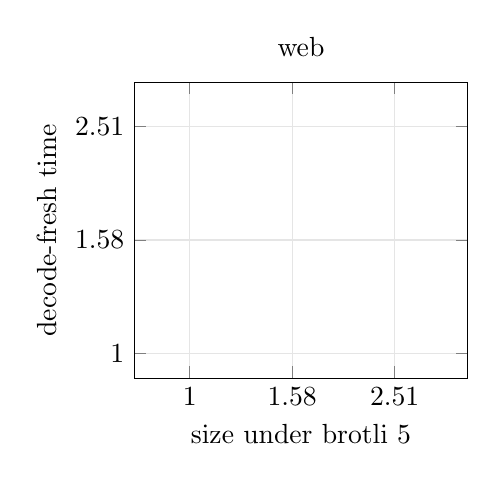
\begin{tikzpicture}
\begin{axis}[width=0.48\linewidth, height=0.44\linewidth, title={web},
  xlabel={size under brotli 5}, ylabel={decode-fresh time},
  xmode=log, ymode=log, log ticks with fixed point,
  nodes near coords, point meta=explicit symbolic,
  every node near coord/.append style={font=\tiny, anchor=west},
  grid=major, grid style={gray!20}, enlarge x limits=0.25]
\IfFileExists{\tables/fig-tradeoff-web.dat}{
  \addplot[only marks, mark=*, mark size=1.5pt] table[x=br5, y=decode, meta=format]{\tables/fig-tradeoff-web.dat};}{}
\end{axis}
\end{tikzpicture}\hfill
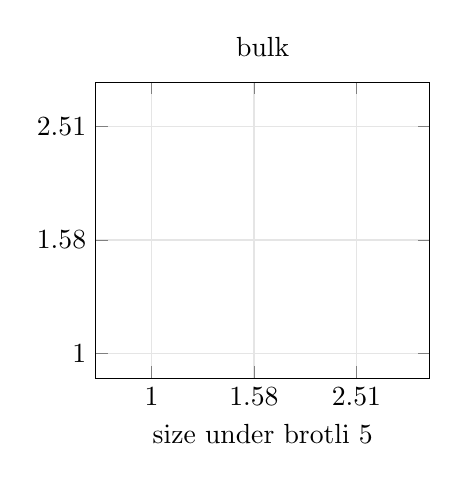
\begin{tikzpicture}
\begin{axis}[width=0.48\linewidth, height=0.44\linewidth, title={bulk},
  xlabel={size under brotli 5},
  xmode=log, ymode=log, log ticks with fixed point,
  nodes near coords, point meta=explicit symbolic,
  every node near coord/.append style={font=\tiny, anchor=west},
  grid=major, grid style={gray!20}, enlarge x limits=0.25]
\IfFileExists{\tables/fig-tradeoff-bulk.dat}{
  \addplot[only marks, mark=*, mark size=1.5pt] table[x=br5, y=decode, meta=format]{\tables/fig-tradeoff-bulk.dat};}{}
\end{axis}
\end{tikzpicture}
\caption{Size against decode time, both against JSON's, per format and
regime (geometric means; each format over the cases it carries). Down and to
the left is better on both.}
\label{fig:tradeoff}
\end{figure}

\FloatBarrier
\subsection{\colbin{} against each format on common cases}
\label{sec:versus}

\begin{table}[t]
\centering\footnotesize
\resulttable{versus-web}
\caption{Web regime: \colbin{}'s number over each other format's, as a
geometric mean over the cases both carry, and in small type the number of
those cases in which \colbin{}'s is strictly lower. Below 1, \colbin{} is
smaller or faster.}
\label{tab:versus-web}
\end{table}

\begin{table}[t]
\centering\footnotesize
\resulttable{versus-bulk}
\caption{Bulk regime: \colbin{} against each other format on common cases.}
\label{tab:versus-bulk}
\end{table}

The tables above give each format a mean over its own cases.
Tables~\ref{tab:versus-web} and~\ref{tab:versus-bulk} remove that
difference: each row compares \colbin{} with one format on exactly the cases
both carry, and counts the cases \colbin{} wins outright. In the web regime
\colbin{} is smaller than Protocol Buffers under brotli 5 in
\result{vs.web.protobuf.br5.wins} of \result{vs.web.protobuf.br5.n} cases
(mean ratio \result{vs.web.protobuf.br5}) and smaller than Avro in
\result{vs.web.avro.br5.wins} of \result{vs.web.avro.br5.n}
(\result{vs.web.avro.br5}). It encodes faster than \fmt{vtprotobuf} in
\result{vs.web.vtprotobuf.encode.wins} of
\result{vs.web.vtprotobuf.encode.n} cases and faster than generated
MessagePack in \result{vs.web.msgpack.encode.wins} of
\result{vs.web.msgpack.encode.n}, and decodes faster than each in
\result{vs.web.vtprotobuf.decode-fresh.wins} and
\result{vs.web.msgpack.decode-fresh.wins} cases. The rows for \colbin{}'s
own variants measure its options: field tags against none, \fmt{packed5},
and the embedded schema section.

\FloatBarrier
\subsection{What a message is made of}
\label{sec:composition}

\begin{table}[t]
\centering\footnotesize
\resulttable{composition}
\caption{\colbin{} messages by regime and dataset: struct rows at any depth,
the share of them written as table rows, the share of the message's bytes
that are tables, and the schema section (median bytes per case; median
share of the message it describes; the section is not part of the message
unless embedded). The last column is the median of bytes per leaf value.}
\label{tab:composition}
\end{table}

Table~\ref{tab:composition} shows how much of each dataset the table layout
reaches. The tabular datasets are tables almost entirely, by construction.
SchemaStore's documents hold \result{composition.web.schemastore.rows}
struct rows in total, \result{composition.web.schemastore.table-rows}\,\% of
them in tables: on that dataset \colbin{} is a row format, and its results
there measure the row format alone.

The schema section, when embedded, costs its size once per message: a
median of \result{composition.web.publicbi.schema-bytes} bytes on Public BI,
\result{composition.web.publicbi.schema-share}\,\% of the message, and
\result{composition.web.schemastore.schema-bytes} bytes on SchemaStore's
typed documents, where it is \result{composition.web.schemastore.schema-share}\,\%
of a message that is itself tens of bytes. A self-describing message is
nearly free for a table and more than doubles a small document, which is
why a stream of small messages should send the section once per connection
instead. \recheck{``more than doubles'' needs the SchemaStore share above 100}

\FloatBarrier
\subsection{Ablations}
\label{sec:ablations}

Two constants shape the table layout: the row count at which a slice
becomes a table, and the rule that picks a column's transform. Both are
compile-time constants in \colbin{}; a build tag of the library, used only
here, turns them into variables. The ablations measure size only, since
that build is not the one to time, and every variant is checked to decode
back to the original value.

\begin{table}[t]
\centering\footnotesize
\resulttable{ablation-threshold}
\caption{Table threshold: \colbin{}'s size with the threshold at 2, 4, 16
and 32 rows over its size at the default of 8, as written and under brotli
5 (geometric mean over cases).}
\label{tab:ablation-threshold}
\end{table}

\paragraph{Threshold (Table~\ref{tab:ablation-threshold}).} The threshold
matters only for slices near it. The tabular cases are single tables of
thousands of rows and do not move. The cases that do are those with many
short slices: TPC-H's nested orders, whose line items number one to seven
per order, and SchemaStore's documents.
\recheck{state the direction and size of the effect at 2, 4, 16, 32 once the
full ablation has run; run1 has none}

\begin{table}[t]
\centering\footnotesize
\resulttable{ablation-codec}
\caption{Column transform: \colbin{}'s size with every integer column forced
to raw, delta or frame of reference, over its size with the transform
chosen per column, as written and under brotli 5.}
\label{tab:ablation-codec}
\end{table}

\paragraph{Column transform (Table~\ref{tab:ablation-codec}).} Forcing one
transform on every column shows what the per-column choice is worth, and
what the transforms are worth at all: the \emph{raw} column is bit-packing
alone. \recheck{report the cost of raw and of each single transform against
the scored choice, as written and under brotli, by dataset}

\paragraph{The other options.} The effect of field tags, of \fmt{packed5}
and of embedding the schema is read from the variants in the main tables:
in the web regime \fmt{colbin-untagged} is at
\result{size.web.colbin-untagged.raw} of JSON as written against
\result{size.web.colbin.raw} for the tagged default (over the cases each
carries; Table~\ref{tab:versus-web} compares them on common cases),
\fmt{colbin+packed5} at \result{size.web.colbin+packed5.raw} as written and
\result{size.web.colbin+packed5.br5} under brotli 5, and \fmt{colbin-json}
at \result{size.web.colbin-json.raw}. Packing strings at five bits a
character saves bytes as written and gives them back under compression,
which does better on plain text than on packed text; it is off by default
for that reason. \recheck{packed5: confirm raw gain and br5 loss}

\FloatBarrier
\section{Limitations}
\label{sec:limitations}

\subsection{Where \colbin{} loses or ties}

\paragraph{Single records, against Avro.} On records with no table in
them \colbin{} is a row format with one byte of header per field, and Avro,
which writes no header at all, is smaller as written: on SchemaStore
\colbin{} against Avro is \result{vs.datasets.schemastore.avro.raw.factor}
as written and \result{vs.datasets.schemastore.avro.gzip.factor} under
gzip, smaller in
\result{vs.datasets.schemastore.avro.gzip.wins} of
\result{vs.datasets.schemastore.avro.gzip.n} documents. Avro pays for this
with a reader that must have the writer's exact schema.

\paragraph{Time on single records, against generated code.} On SchemaStore
\colbin{}'s encode time against \fmt{vtprotobuf}'s is
\result{vs.datasets.schemastore.vtprotobuf.encode.factor} and against
generated MessagePack's
\result{vs.datasets.schemastore.msgpack.encode.factor}; it encodes
faster in \result{vs.datasets.schemastore.vtprotobuf.encode.wins} of
\result{vs.datasets.schemastore.vtprotobuf.encode.n} and
\result{vs.datasets.schemastore.msgpack.encode.wins} of
\result{vs.datasets.schemastore.msgpack.encode.n} documents, and to decode it is
\result{vs.datasets.schemastore.msgpack.decode-fresh.factor} against
generated MessagePack and
\result{vs.datasets.schemastore.flatbuffers.decode-fresh.factor} against
FlatBuffers. Straight-line generated code beats a plan interpreted
per field on a message of a few fields; the columnar path is what makes up
the difference on tables.

\paragraph{Access without decoding.} \colbin{} must decode a message to read
one field of it. Arrow and FlatBuffers read a column in place and are faster
at it by orders of magnitude (Section~\ref{sec:results}).

\paragraph{Data with nothing to exploit.} A column of random 64-bit values
costs its eight bytes a value plus a width byte per block; strings are not
compressed at all by the default format. A table that is mostly long,
distinct strings is the size of its strings in any format.

\subsection{What the evaluation does not cover}

\paragraph{The author evaluates his own format.} The format, the harness and
the choices below are one person's, and a reader should weigh the results
accordingly. Four things bound the choices. The data is third-party, and the
Go types of \result{cases.categories.bulk} bulk and
\result{cases.categories.web-tables} web tables are generated from the
sources' \code{CREATE TABLE} statements; only SchemaStore's are written by
hand (below). Every other format's schema is generated from those same
types, so no format is given a type of its own. Each library is called with
its default options and through the interface its documentation gives for a
hot path: generated code encodes into the caller's buffer, the FlatBuffers
builder is reused, \colbin{} runs through a codec handle built once per
type, and converting between a generated type and the Go struct is not
timed. And the departures from a default are few and stated here: CBOR's
decoder has its limits on array and map sizes raised, which a table of
$10^5$ rows exceeds; Arrow's buffers are not compressed, so that its size as
written is not a compressed one; \fmt{gob} writes one message per encoder,
and so describes its types in every message. Two choices remain that favour
\colbin{}. The rule for types, decimals and money as integer minor units and
dates as integer days, keeps the sources' exact types exact, but it puts
most values where an integer codec works, which is \colbin{}'s strength; the
evaluation does not measure a schema that keeps them as floats or strings.
And the
libraries, one or two per format, were chosen by the author as the ones in
common use in Go; another implementation of the same format would time
differently.

\paragraph{One language and one implementation per format.} All measurements
are of Go implementations. A format's speed is its implementation's: the
two implementations of Protocol Buffers and of MessagePack measured here
differ by more than most pairs of formats do. The sizes carry over to other
languages; the times do not.

\paragraph{Two machines, both x86-64 and of one vendor.} The main times come from one server
processor model, in four cloud container instances of the same shape (one
per dataset), whose clock the host controls and whose cache and memory
bandwidth other tenants share. A summary over a regime pools cases measured
in different instances; a ratio on one case never does. We measured that
clock rather than fixed it (Section~\ref{sec:machine}). Absolute times there
were not repeatable to 3\,\% between two passes; the ratios this paper
reports were, to within \result{repeat.ratio-worst}\,\%, and differences
below about 4\,\% should not be read as differences. The second machine, a
laptop with its clock fixed (Section~\ref{sec:second-machine}), shows which
conclusions survive a change of processor, but it is a single unit of a
single model, and two machines are not a population. Both are x86-64
processors of AMD, one generation apart: no Intel processor and no arm64
machine was measured.

\paragraph{Datasets not covered.} Real floats and timestamps are
represented by Public BI only. No dataset here was assembled by a third
party specifically to compare serialization formats except SchemaStore's
corpus, and the evaluation is not validated against an existing third-party
benchmark suite.

\paragraph{Synthetic distributions.} TPC-H and TPC-DS draw values from
near-uniform distributions, which under-represent the skew and correlation
of real data~\cite{vogelsgesang2018getreal}. They are reported per dataset
so that Public BI, which is real, can be read on its own
(Section~\ref{sec:by-dataset}).

\paragraph{Hand-written types for SchemaStore.} The Go structs for the 27
SchemaStore documents were written by the author, from the corpus's
Protocol Buffers schemas. Choices of integer width, of pointer or value, and
of field numbering affect every schema-driven format, not only \colbin{},
but they are choices. The artifact also measures each document as a
\code{map[string]any}, which involves none; only the schemaless formats and
Protocol Buffers (through \code{google.protobuf.Value}) can carry that, so it
compares \colbin{} with a few formats on cases the others do not have, and
it is not reported here.
\result{coverage.web.colbin.na} documents cannot be given a type \colbin{}
carries and are reported as not applicable, which removes them from
\colbin{}'s comparisons; the other formats' means against JSON
(Appendix~\ref{sec:against-json}) are over them.

\paragraph{gob.} \fmt{gob} omits zero values and does not distinguish a nil
pointer from a pointer to zero, so it does not round-trip a table with a
nullable column that holds a zero:
\result{coverage.web.gob.lossy} of \result{cases.web} web cases and
\result{coverage.bulk.gob.lossy} of \result{cases.bulk} bulk cases. On those
it is sized but not timed, so its timing means are over fewer cases, and
they are the cases without nullable columns. Its sizes also depend on what
the process encoded before, because \fmt{gob} assigns type identifiers per
process in order of first use; all cases of a run are sized in one process,
in a fixed order, and a different selection of cases gives sizes that
differ by up to a dozen bytes a message. Both machines sized one dataset
per process, so their sizes agree on every case reported here.

\paragraph{Stability of the format.} \colbin{} is at version
\result{machine.colbin-version}, before 1.0, with no compatibility promise
between minor versions. The numbers are for that version.

\paragraph{Not measured.} The cost of the first use of a type, when the
encoding plan is built, is not measured: every time in this paper is of a
warmed-up process. Memory is reported for decode only
(Section~\ref{sec:memory}), as what an operation allocates, not as what the
process holds. Schema evolution is described and tested for behaviour
(Section~\ref{sec:evolution}), not for cost.

\section{Conclusion}
\label{sec:conclusion}

A serialization format does not have to choose between being a row format
that is cheap for a small message and a columnar one that is compact for a
table. \colbin{} is both: it decides per slice, at encode time, with a
threshold of eight rows, and applies to the columns a small set of integer
transforms and byte-aligned bit-packing that cost little on a short column
and pay increasingly on a long one. It needs no schema file and no generated
code, and a message that embeds its schema can be read as JSON by a reader
that has never seen its type.
The evaluation shows where this pays and where it does not, on data the
author did not design, and the artifact lets a reader check each number.

\section{Code and data availability}
\label{sec:availability}

The benchmarks, dataset scripts, checksums, raw results and the source of
this paper are available at the tag \code{paper-v1} of its repository:
\begin{itemize}
\item repository: \url{https://github.com/ivanjoz/colbin-benchmarks/tree/paper-v1}
\item commit of the tag: \code{625207318491c32bf36d2894117e6a22697443ba}
\item archive: \url{https://doi.org/10.5281/zenodo.24261124}
\item main machine measured at: \code{\result{machine.commit}},
  \colbin{} \result{machine.colbin-version}
\item second machine measured at: \code{\result{laptop.machine.commit}},
  \colbin{} \result{laptop.machine.colbin-version}
\item \colbin{}: \url{https://github.com/ivanjoz/colbin}
\end{itemize}
The raw results of both machines are in the repository,
\code{results/paper-v1} and \code{results/paper-v1-laptop}.
Running \code{./reproduce.sh} at the tag downloads and verifies the
datasets, runs every measurement, and regenerates every table and figure of
this paper; the tables and the numbers quoted in the text are generated
files, not transcriptions.


\bibliographystyle{plain}
\bibliography{related-work}

\appendix
\section{Each format against JSON, by regime}
\label{sec:against-json}

The tables of this appendix give every format against JSON on the same case,
as a geometric mean over the cases the format carries, with the web and bulk
regimes apart; below 1 is smaller or faster than JSON. Because formats
differ in the cases they carry, two formats' means here are not directly
comparable; Section~\ref{sec:results} compares \colbin{} with each format on
the cases both carry. Tables~\ref{tab:versus-web} and~\ref{tab:versus-bulk}
do the same by regime, with \colbin{}'s own variants.

\begin{table}[ht]
\centering\small
\resulttable{sizes-web}
\caption{Web regime: message size against JSON's, as written (\emph{raw})
and under each compressor, both sides compressed alike. $\dagger$: cases
where the format writes zero bytes are left out of the mean.}
\label{tab:sizes-web}
\end{table}

\begin{table}[ht]
\centering\small
\resulttable{sizes-bulk}
\caption{Bulk regime: message size against JSON's.}
\label{tab:sizes-bulk}
\end{table}

\begin{table}[ht]
\centering\footnotesize
\resulttable{sizes-datasets-web}
\caption{Web regime by dataset: size against JSON's, as written and under
gzip.}
\label{tab:sizes-datasets-web}
\end{table}

\begin{table}[ht]
\centering\small
\resulttable{times-web}
\caption{Web regime: time against JSON's for the same operation
(\result{time.web.cases} cases; access against JSON's decode-fresh, on the
\result{time.web.access.cases} cases that have an access aggregate).}
\label{tab:times-web}
\end{table}

\begin{table}[ht]
\centering\small
\resulttable{times-bulk}
\caption{Bulk regime: time against JSON's for the same operation
(\result{time.bulk.cases} cases).}
\label{tab:times-bulk}
\end{table}

\begin{table}[ht]
\centering\footnotesize
\resulttable{versus-web}
\caption{Web regime: \colbin{}'s number over each other format's, as a
geometric mean over the cases both carry, and in small type the number of
those cases in which \colbin{}'s is strictly lower. Below 1, \colbin{} is
smaller or faster.}
\label{tab:versus-web}
\end{table}

\begin{table}[ht]
\centering\footnotesize
\resulttable{versus-bulk}
\caption{Bulk regime: \colbin{} against each other format on common cases.}
\label{tab:versus-bulk}
\end{table}

\begin{figure}[ht]
\centering
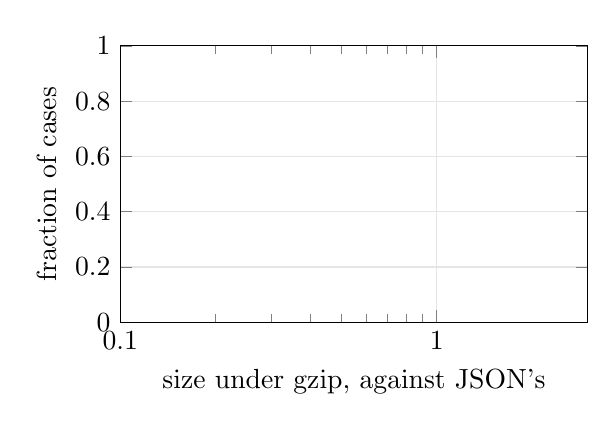
\begin{tikzpicture}
\begin{axis}[width=0.62\linewidth, height=0.42\linewidth,
  xlabel={size under gzip, against JSON's}, ylabel={fraction of cases},
  xmode=log, log ticks with fixed point, xmin=0.1, xmax=3, ymin=0, ymax=1,
  legend pos=outer north east, legend style={font=\footnotesize, draw=none},
  cycle list name=color list, grid=major, grid style={gray!20}]
\distcurve{very thick, black}{fig-dist-web-gzip-colbin}{colbin}
\distcurve{thick, blue}{fig-dist-web-gzip-protobuf}{protobuf}
\distcurve{thick, red}{fig-dist-web-gzip-avro}{avro}
\distcurve{thick, orange}{fig-dist-web-gzip-msgpack}{msgpack}
\distcurve{thick, teal}{fig-dist-web-gzip-arrow}{arrow}
\distcurve{thick, gray}{fig-dist-web-gzip-flatbuffers}{flatbuffers}
\end{axis}
\end{tikzpicture}
\caption{Web regime: the distribution over cases of each format's size under
gzip against JSON's under gzip. A curve to the left is smaller; each
format's curve is over the cases it carries.}
\label{fig:dist-size}
\end{figure}

\begin{figure}[ht]
\centering
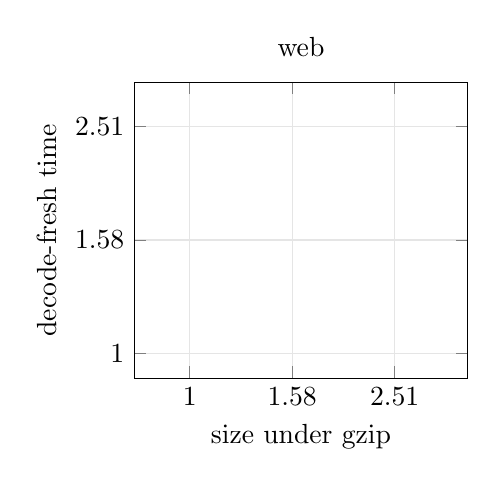
\begin{tikzpicture}
\begin{axis}[width=0.48\linewidth, height=0.44\linewidth, title={web},
  xlabel={size under gzip}, ylabel={decode-fresh time},
  xmode=log, ymode=log, log ticks with fixed point,
  nodes near coords, point meta=explicit symbolic,
  every node near coord/.append style={font=\tiny, anchor=west},
  grid=major, grid style={gray!20}, enlarge x limits=0.25]
\IfFileExists{\tables/fig-tradeoff-web.dat}{
  \addplot[only marks, mark=*, mark size=1.5pt] table[x=gzip, y=decode, meta=format]{\tables/fig-tradeoff-web.dat};}{}
\end{axis}
\end{tikzpicture}\hfill
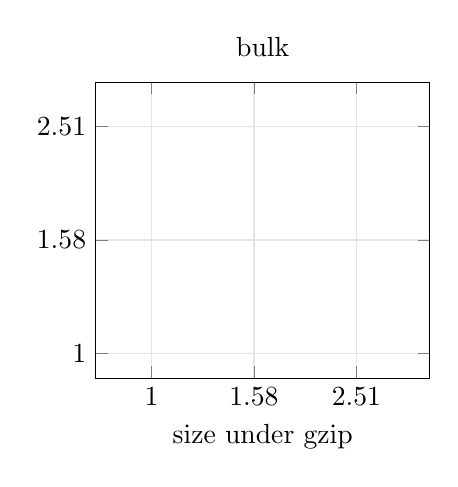
\begin{tikzpicture}
\begin{axis}[width=0.48\linewidth, height=0.44\linewidth, title={bulk},
  xlabel={size under gzip},
  xmode=log, ymode=log, log ticks with fixed point,
  nodes near coords, point meta=explicit symbolic,
  every node near coord/.append style={font=\tiny, anchor=west},
  grid=major, grid style={gray!20}, enlarge x limits=0.25]
\IfFileExists{\tables/fig-tradeoff-bulk.dat}{
  \addplot[only marks, mark=*, mark size=1.5pt] table[x=gzip, y=decode, meta=format]{\tables/fig-tradeoff-bulk.dat};}{}
\end{axis}
\end{tikzpicture}
\caption{Size against decode time, both against JSON's, per format and
regime (geometric means; each format over the cases it carries). Down and to
the left is better on both.}
\label{fig:tradeoff}
\end{figure}


\end{document}
